\chapter{Resultados y Análisis}\label{chap:resultados}

En este capítulo se deben presentar y analizar los resultados de la tesis. Es importante seleccionar aquellos resultados suficientemente relevantes para validar la hipótesis y demostrar el cumplimiento de los objetivos. Los resultados menos relevantes pueden ser incluidos en los anexos (Apéndice \ref{chap:AnexoA} en esta plantilla). Es importante referenciar estos resultados anexos en el texto, por ejemplo: ``Algunos resultados relacionados a (...) se pueden encontrar en el Anexo \ref{chap:AnexoA}''.

\begin{figure}[h]
    \centering
    \begin{subfigure}{\textwidth}
        \centering
        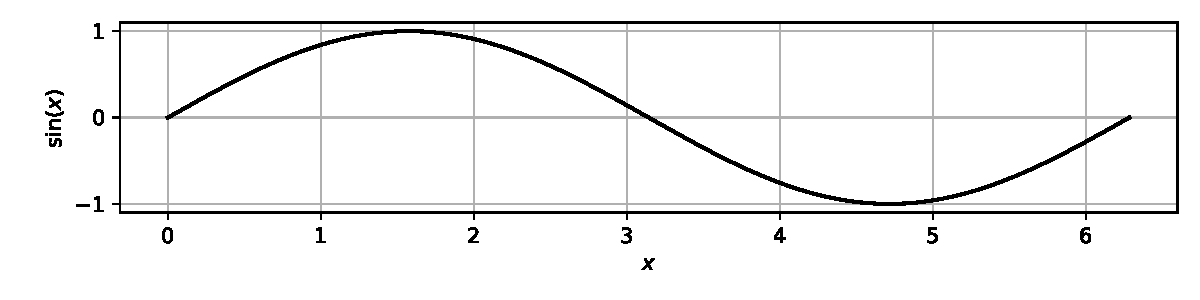
\includegraphics[width=\textwidth]{Figuras/Resultados/seno.pdf}
        \caption{Señal seno.}
        \label{fig:seno}
    \end{subfigure}
    \begin{subfigure}{\textwidth}
        \centering
        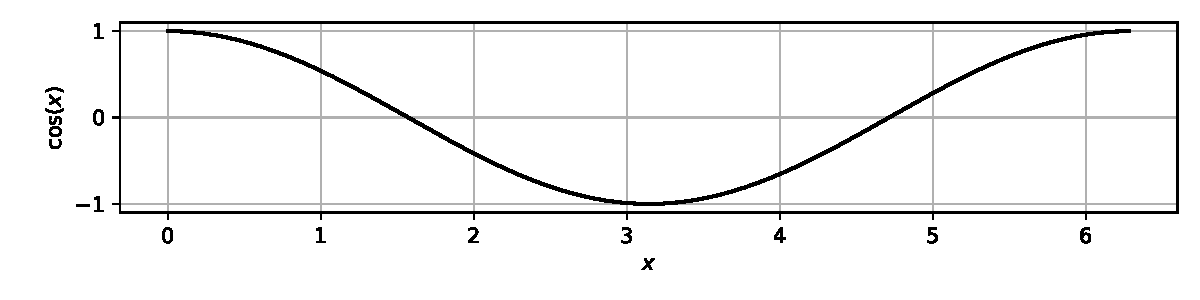
\includegraphics[width=\textwidth]{Figuras/Resultados/coseno.pdf}
        \caption{Señal coseno.}
        \label{fig:coseno}
    \end{subfigure}
    \caption{Ejemplos de señales trigonométricas.\label{fig:senales}}
\end{figure}

Las tablas y figuras utilizadas deben ser precisas y concisas. Es importante que cada resultado sea analizado inmediatamente al momento de ser presentado, evitando acumular figuras o tablas para analizarlas todas al final. En ocasiones, al presentar gráficos similares o provenientes de un mismo experimento, puede ser útil agruparlos en una misma figura, como se muestra en la figura \ref{fig:senales}. De esta manera, es posible referenciar la figura completa o una subfigura específica de forma independiente, por ejemplo la figura \ref{fig:seno}. Para cerrar este capítulo, puede ser útil incluir una sección que recapitule los principales hallazgos; sin embargo, esta no debe denominarse ``Resumen'', dado que la tesis ya cuenta con uno en la sección inicial.